%%%%%%%%%%%%%%%%%%%%%%%%%%%%%%%%%%%%%%%%%
%
% (c) 2018 by Jennifer Laaser
%
% This work is licensed under the Creative Commons Attribution-NonCommercial-ShareAlike 4.0 International License. To view a copy of this license, visit http://creativecommons.org/licenses/by-nc-sa/4.0/ or send a letter to Creative Commons, PO Box 1866, Mountain View, CA 94042, USA.
%
% The current source for these materials is accessible on Github: https://github.com/jlaaser/quantum-exercises
%
%%%%%%%%%%%%%%%%%%%%%%%%%%%%%%%%%%%%%%%%%

\section*{Quantum States: Analogies to Functions and Vectors\sectionmark{Exercise: States, Functions, \& Vectors}}

	Quantum states are abstract, but we can get some intuition for their properties by drawing \emph{analogies} to functions and vectors.

	\begin{questions}
	
		\question Use your knowledge about functions and vectors to predict what expression should go in each of the blank cells in this table. A few of the lines are filled out to get you started.
		
			%\vspace{-0.2in}
			\begin{center}
				\renewcommand{\arraystretch}{1.5}
			\begin{tabular}{|C{2in}| C{2in} | C{2in}|}
				\hline
				
				\textbf{Functions} 
				& \textbf{Vectors}  
				& \textbf{Quantum States}
				\\
				\hline
				
				$f(x)$
				& $\vec v = \begin{pmatrix} v_1 \\ v_2 \\ v_3\end{pmatrix}$
				& $\ket{\alpha}$
				\\
				\hline
				
				$f^*(x)$
				& $\vec v\,^\dag = \begin{pmatrix} v_1^* & v_2^* & v_3^*\end{pmatrix}$
				& $\bra{\alpha}$
				\\
				\hline
				
				$h(x) = f(x) + g(x)$
				& $\vec w = \vec u + \vec v$
				& $\ket\gamma = \ket \alpha + \ket \beta$
				\\
				\hline
				
				& $\left( c\vec v \right)^\dag = c^* \vec v\,^\dag$
				& \vspace{0.75in}
				\\
				\hline
				
				$\int_{-\infty}^\infty dx\, f^*(x) f(x)$
				& $\vec v\,^\dag \vec v$
				& $\braket{\alpha|\alpha}$
				\\
				\hline
				
				&$\left(\vec u\,^\dag \vec v\right)^* = \vec v\,^\dag \vec u$
				& \vspace{0.75 in}
				\\
				\hline
				
				$\int_{-\infty}^\infty dx\, f^*(x) f(x) \geq 0$
				&
				& \vspace{0.75 in}
				\\
				\hline
				
				& \vspace{0.75 in}
				&
				$\braket{\beta|c|\alpha} = c \braket{\beta|\alpha}$
				\\
				\hline
				
				
			\end{tabular}
			\end{center}
		
		\emph{Note: we are using a very general notation here that allows vectors and functions to have complex values. If $\vec u$ and $\vec{v}$ are purely real, however, then $\vec u \,^\dag \vec v$ is just equal to the dot product $\vec u \cdot \vec v$ - I encourage you to try working through this if you are unsure about why it should be true.}
		
		\contdnewpg
		
		\newpage
		\question If $\vec a$ is a vector, then $\vec a\,^\dag \vec a$ gives the square of the length of the vector.
			\begin{parts}
				\part Why is it always true that $\vec a\,^\dag \vec a > 0$?
					\begin{solution}[1.5in]
					\end{solution}
				
				\part In this context, how would you interpret $\braket{\alpha|\alpha}$?
					\begin{solution}[1.5in]
					\end{solution}
			\end{parts}
		\question If $\vec a$ and $\vec b$ are vectors, then the \emph{projection} of $\vec{b}$ onto $\vec{a}$ is
			\begin{center}
			\begin{minipage}{0.4\textwidth}
					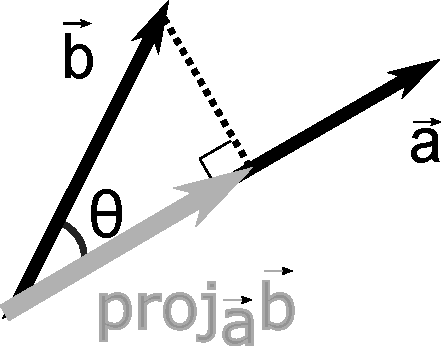
\includegraphics[width=0.7\textwidth]{includes/states-funcs-vecs-FIGURES/vector_projection.pdf}
			\end{minipage}
			\begin{minipage}{0.4\textwidth}
					\begin{align*}
						proj_{\vec a}\vec{b} &= \left(\text{length}\right)\left(\text{direction}\right) \\
						&= \left(|\vec{b}|cos(\theta)\right)\left( \frac{\vec{a}}{|\vec{a}|}\right) \\
							&= \left(|\vec{b}|\frac{\vec{a}\,^\dag\vec{b}}{|\vec{a}||\vec{b}|}\right)\left( \frac{\vec{a}}{|\vec{a}|}\right) \\
							&= \frac{\vec a\,^\dag \vec{b}}{|\vec{a}|^2}\vec{a} 
					\end{align*}
			\end{minipage}
			\end{center}
		
			\vspace{0.2in}
			In this context, how would you interpret the following expression? 
			\begin{equation*}		
				\frac{\braket{\alpha|\beta}}{\braket{\alpha|\alpha}}\ket{\alpha}
			\end{equation*}
			
			\begin{solution}[1.7in]
			\end{solution}

	\end{questions}

	\stophere